% Plano inclinado com diagrama de forças
% Feito para o ÉguaTeX (eguatex.com.br). Uso livre (CC0 1.0).
%
% Compile e pronto: sai só a figura, em PDF.
% Para pôr no seu trabalho, use o PDF com \includegraphics ou copie
% o bloco tikzpicture para dentro de uma figure.
%
% O peso P se divide em duas partes: P sen(theta), ao longo da rampa,
% e P cos(theta), contra a rampa. A normal N equilibra P cos(theta).
\documentclass[tikz,border=4pt]{standalone}
\usepackage[T1]{fontenc}
\usepackage{lmodern}
\usepackage{amsmath}
\usetikzlibrary{calc, angles, quotes, patterns.meta}

\colorlet{corPeso}{red!75!black}
\colorlet{corComp}{red!75!black}
\colorlet{corNormal}{blue!75!black}
\colorlet{corAtrito}{green!45!black}

\begin{document}
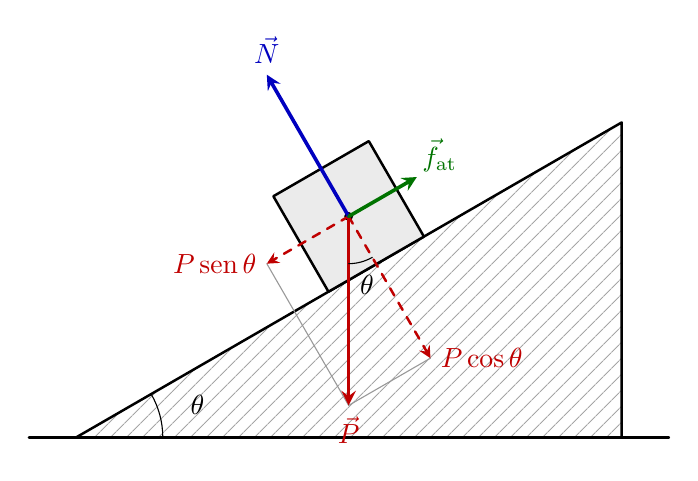
\begin{tikzpicture}[line cap=round, line join=round, >=stealth,
  forca/.style={->, line width=1.3pt},
  comp/.style={->, line width=0.9pt, dashed}]

% Mude estes números e o desenho e os rótulos acompanham.
\def\ang{30}     % inclinação da rampa, em graus (entre 10 e 50)
\def\rampa{8}    % comprimento da rampa, em cm
\def\pos{0.55}   % onde fica o bloco, de 0 (base) a 1 (topo)
\def\lado{1.4}   % lado do bloco, em cm
\def\peso{2.4}   % tamanho da seta do peso, em cm
\def\atrito{1.0} % tamanho da seta do atrito, em cm (0 para tirar)

\pgfmathsetmacro{\cs}{cos(\ang)}
\pgfmathsetmacro{\sn}{sin(\ang)}

% rampa e chão
\coordinate (A) at (0,0);
\coordinate (B) at ({\rampa*\cs},0);
\coordinate (C) at ({\rampa*\cs},{\rampa*\sn});
\fill[pattern={Lines[angle=45, distance=4pt, line width=0.4pt]}, pattern color=black!35]
  (A) -- (B) -- (C) -- cycle;
\draw[line width=0.9pt] (A) -- (B) -- (C) -- cycle;
\draw[line width=0.9pt] (-0.6,0) -- ($(B)+(0.6,0)$);
\pic[draw, "$\theta$", angle eccentricity=1.45, angle radius=1.1cm] {angle=B--A--C};

% bloco, apoiado na rampa
\begin{scope}[rotate=\ang]
  \draw[line width=0.9pt, fill=black!8]
    ({\pos*\rampa-\lado/2},0) rectangle ({\pos*\rampa+\lado/2},\lado);
  \coordinate (G) at ({\pos*\rampa},{\lado/2});
\end{scope}
\fill (G) circle[radius=1.6pt];

% peso e suas componentes
\coordinate (P)  at ($(G)+(0,-\peso)$);
\coordinate (Pc) at ($(G)+({\peso*\cs*\sn},{-\peso*\cs*\cs})$);
\coordinate (Ps) at ($(G)+({-\peso*\sn*\cs},{-\peso*\sn*\sn})$);
\draw[black!40] (P) -- (Pc);
\draw[black!40] (P) -- (Ps);
\draw[comp, corComp] (G) -- (Pc) node[right] {$P\cos\theta$};
\draw[comp, corComp] (G) -- (Ps) node[left] {$P\operatorname{sen}\theta$};
\draw[forca, corPeso] (G) -- (P) node[below] {$\vec{P}$};
\pic[draw, "$\theta$", angle eccentricity=1.5, angle radius=0.6cm] {angle=P--G--Pc};

% normal e atrito
\draw[forca, corNormal] (G) -- ($(G)+({-\peso*\cs*\sn},{\peso*\cs*\cs})$) node[above] {$\vec{N}$};
\draw[forca, corAtrito] (G) -- ($(G)+({\atrito*\cs},{\atrito*\sn})$) node[above right=-2pt] {$\vec{f}_{\mathrm{at}}$};
\end{tikzpicture}
\end{document}
